
%%%%%%%%%%%%%%%%%%%%%%%%%%%%%%%%%%%%%%%%%%%%%%%%%%%%%%%%%%%%%%%%%%%%%%%%%%%%%%%%
%%%%%%%%%%%%%%%%%%%%%%%%%%%%%%%%%%%%%%%%%%%%%%%%%%%%%%%%%%%%%%%%%%%%%%%%%%%%%%%%
\section{Musicalidade, sentir ou entender a música?}
Seguindo a Definição \ref{def:Musicalidade}, podemos inferir como entender a musicalidade na dança.
\begin{definition}[Musicalidade na dança] 
\index{Musicalidade}
\label{def:MusicalidadeNaDanca}
Esta acontece, quando o dançarino tem um estado de ``sensibilidade'' ou ``conhecimento'' para contemplar ou entender a música 
e assim quando este dança ``demostrar'' uma coerência entre a música e o que se está dançando.
\end{definition}

Porém temos um choque de paradigmas, na definição, para atingir um mesmo objetivo que é ser musical.
Podemos \hyperref[ref:emotionsentimental]{\textbf{sentir}} ou 
\hyperref[subsec:tecnica-sentimentos]{\textbf{conhecer}}; o que é equivalente a dizer que:
\begin{itemize} 
\item podemos saber por intuição e sensibilidade sem entender o porquê, ou
\item podemos saber entendendo mediante o conhecimento adquirido pelo raciocínio e o estudo da música e sua percepção.
\end{itemize}



Neste sentido, para adquirir esta coerência com a música, 
muitos professores indicam que o dançarino deve ``escutar e sentir a música'';
nesse aspecto, argumento que a frase é correta e coincide em parte com 
as Definições \ref{def:Musicalidade} e \ref{def:MusicalidadeNaDanca};
porém a frase  é pedagogicamente pouco favorável para o estudante.
Assim, eu ressaltaria que a musicalidade a nível de ensino se adquire,
estudando e entendendo a música e como esta é percebida pelo nosso cérebro, e não só sentindo-a.
 
Para fundamentar minha argumentação, acredito interessante expor o Exemplo \ref{ex:srinivasa}. 
\begin{example}[O matemático que sentia os números:]
\label{ex:srinivasa}
Imaginemos que conhecemos ao matemático ``Srinivasa Aiyangar Ramanujan'';
um prodígio matemático autodidata \cite[pp. 1]{kanigel2016man}, indiano, que 
realizou muitas contribuições à matemática\footnote{Existe 
um filme chamado `` The Man Who Knew Infinity'' (2015) ou 
``O Homem que Viu o Infinito'' em português, que conta a história de vida de Srinivasa Aiyangar Ramanujan.};
explicamos a ele um problema  matemático, 
como por exemplo uma equação,
e  lhe pedimos uma resposta ou solução. 
Então Srinivasa, muito amavelmente, 
observaria um instante o problema e nos daria a solução imediatamente.
Nós surpreendidos pela velocidade e o mínimo esforço na resposta,
perguntaríamos: Como você obteve esse resultado? Então ele responderia \cite[pp. 235]{kanigel2016man}:\\

%\begin{citando}
%Immediately I heard the problem 
%it was clear that the solution should obviously be a continued fraction; 
%I then thought, Which continued  fraction? And the answer came to my mind.
%\end{citando}
%\begin{citando}
``No momento em que escutei o problema, 
foi claro pra mim que a resposta devia ser obviamente uma fração continua; 
e então pensei, ¿Qual fração continua? e a resposta chegou a minha mente''.\\
%\end{citando}

Exemplo de fração continua simples:
\begin{equation}
a_{0}+{\frac {1}{a_{1}+{\frac {1}{a_{2}+{\frac {1}{a_{3}+{\frac {1}{\ddots }}}}}}}}
\end{equation}
\end{example}

A resposta que ``Srinivasa'' deu no Exemplo  \ref{ex:srinivasa}, 
é a mesma  que dão as pessoas, quando  dizem que para ter musicalidade ele simplesmente sentiu a música. 
Assim, esta aproximação ao problema é só eficiente, para pessoas como Srinivasa, 
que talvez tenham uma ``inspiração divina'', 
ou que já nasceram com esse dom, ou que por uma longa experiencia de vida atingiram 
a \hyperref[ref:CompetenciaInconsciente]{\textbf{competência inconsciente}}, 
e tem implementado por ``hardware'', no encéfalo, entender a matemática ou a música; 
pelo que eles usam a palavra sentir, 
pois conhecem a resposta, porém não sabem como sabem. 

Assim, este tipo de entendimento  pode acontecer em pessoas que observaram muito tempo um ``problema'', 
ou escutaram muito uma ``música'', 
e um dia conseguiram ``sentir'' a resposta. 
Na minha opinião, 
não todos nascemos com esse componente implementado em nosso encéfalo, para perceber e processar por ``hardware'' (sentir) a música; 
e não podemos nos dar o luxo de escutar uma canção indefinidamente até ``sentir'' algo. 
O mais eficiente seria estudar música, 
entender esta baseando-nos em nossa teoria e cruzar esta informação com o que escutamos,
os padrões observados, a melodia, o ritmo, etc. 
Assim, nos podemos criar por ``software'' o que não temos implementado por ``hardware''\footnote{Como no caso do amigo Srinivasa.}, 
derrubando o mito de só ``sentir'' a música e passar a ``entender'' ela;
seguindo assim o natural \hyperref[sec:aprendizagem]{\textbf{ciclo da aprendizagem}}\footnote{O
ciclo da aprendizagem é estudado na Seção \ref{sec:aprendizagem}.}, passando primeiro pela 
\hyperref[ref:CompetenciaConsciente]{\textbf{competência consciente}} 
antes de atingir a  \hyperref[ref:CompetenciaInconsciente]{\textbf{competência inconsciente}}.

Mas isto não quer dizer que sentir música seja equivocado, este é um caminho valido sim;
porém, apontar primeiro a esse alvo, 
pode chegar a ser pouco favorável se temos estudantes baixo nossa responsabilidade, 
que dependem de nós no seu percorrido para chegar a serem musicais; 
pois se nosso entendimento da musicalidade se baseia unicamente em nossas sensações pessoais,
só poderemos indicar a eles que fechem os olhos e sintam a música.


%%%%%%%%%%%%%%%%%%%%%%%%%%%%%%%%%%%%%%%%%%%%%%%%%%%%%%%%%%%%%%%%%%%%%%%%%%%%%%%%%
\subsection{Musicalidade e a teoria da informação}
\label{sec:musicalidadeinfmutua}

%% Exemplo dançar em coerencia com a música ou não
%% Eurythmics - Sweet Dreams (Are Made Of This) (Official Video)

Dançar com musicalidade não é só dançar com o \hyperref[ref:Pulso]{\textbf{pulso}} da música, 
ou na \hyperref[def:Metrica]{\textbf{métrica}},
existem outros aspectos da música, ou de instrumentos isolados, que podemos seguir como 
\begin{inparaitem} 
\item a melodia, 
\item o ritmo,
\item a \hyperref[sub:Articulation]{\textbf{articulação}} das notas, 
\item as \hyperref[sec:texturasmusica]{\textbf{texturas}}, 
\item as \hyperref[sec:Cadencia]{\textbf{cadências}}, 
\item os \hyperref[sec:Motivo]{\textbf{motivos}}, 
\item o \hyperref[sec:fraseio]{\textbf{fraseio}}, 
\item etc.
\end{inparaitem} 
Com todas essas possibilidades, uma pessoa com musicalidade 
incorpora as caraterísticas que considera que são interessantes para 
ser mostradas na sua dança; por exemplo, poderia dançar interpretando a letra da música.

Neste ponto chegamos a uma pregunta; se eu danço usando a letra e faço exatamente o oposto que indica a letra,
estou dançando com musicalidade?
Para poder responder isto, confiantes na nossa afirmação,
primeiro teríamos que nos fazer outra pergunta.
Se eu danço fazendo o oposto de uma caraterística que tenho escolhido na música,
minha dança seria uma função direta dessa caraterística?
Neste caso a resposta seria ``sim'', pois mesmo fazendo o oposto,
nossa dança estaria atrelada à caraterística escolhida na música.
Pelo que podemos afirmar que se dançamos fazendo o oposto a uma caraterística da música, 
estamos sim dançando com musicalidade.
\begin{example}[A criança não-independente:]
Imaginemos que temos baixo nossa responsabilidade a uma criança,
e esta precisa ir a dormir cedo, pelo que lhe indicamos a ela que já deve ir a dormir;
se a criança é obediente vai a dormir, então seus atos estariam em função de nossos comandos,
pelo que poderíamos considerar ela como dependente de nós;
porém se a criança é ``falsamente'' independente (falsamente rebelde), quando indiquemos que deve ir a dormir,
por contradição ela ficará acordada, mesmo sentindo sono, por ter um falso senso de independência.

Nesse caso a criança é dependente de nossas ordens,
pois seus atos estão em função direta do que nos indiquemos.
Um individuo realmente independente, tomaria suas decisões unicamente em função,
do seu próprio analises e conclusões.
Pelo que poderíamos afirmar que no caso da criança falsamente rebelde, esta é dependente da autoridade.
\end{example}

É neste ponto que podemos invocar à ``teoria da informação'' para poder explicar 
ou modelar esta dependência entre nossos movimentos e a música.
Nesta área do conhecimento existem duas definições, que são:
\begin{itemize} 
\item A informação mútua (binária), que mede a informação que tem em comum dois eventos ou variáveis,
sendo 1.0 quando ambas tem completamente a mesma informação,
zero quando ambas variáveis não tem informação em comum, 
e valores intermediários entre zero e 1.0 quando existe entre eles uma porção da informação \cite{reza2012introduction}. 
\item O coeficiente de correlação (Pearson), 
que indica o grau de dependência a favor ou em contra entre dois eventos ou variáveis,
sendo +1.0 quando os eventos crescem juntos, 
-1.0 quando um cresce enquanto outro diminui na mesma proporção,
 zero quando os dois eventos não tem nada em comum, 
e valores intermediários entre -1.0 e +1.0 para graus intermediários de correlação \cite{reza2012introduction}.
\end{itemize} 

Note-se que a informação mútua entre duas variáveis só tem sinal positiva; assim,
se uma variável cresce na mesma proporção que outra diminui, 
a informação mutua será 1.0 pois uma variável é dependente da outra.
\begin{example}
Dadas as variáveis  $X$ e $Y$, se $Y=-X+3$; então,
a informação mutua entre X e Y é igual a $1.0$, e
a correlação entre $X$ e $Y$ é igual a $-1.0$.
\end{example}

Das explicações anteriores podemos deduzir que: as relações entre a música e a dança 
são melhor descritas com a informação mutua  que com a correlação;
pelo que podemos reformular a Definição \ref{def:MusicalidadeNaDanca} usando a informação mutua:
\begin{definition}[Musicalidade na dança seguindo a teoria da informação] 
\index{Musicalidade}
\label{def:MusicalidadeNaDancaIT}
A musicalidade é um termo que indica o grau de informação mutua que existe entre dois eventos: 
\begin{itemize}
\item A música que é percebida.
\item Os movimentos que são executados.
\end{itemize} 
\end{definition}


Se definimos como $M_u$ a uma variável que representa a informação da música, e 
como $M_o$ a uma variável que representa a informação dos movimentos, 
como mostrado na Figura \ref{fig:InfoMutuaMuMo}.
\begin{figure}[!h]
  \centering
    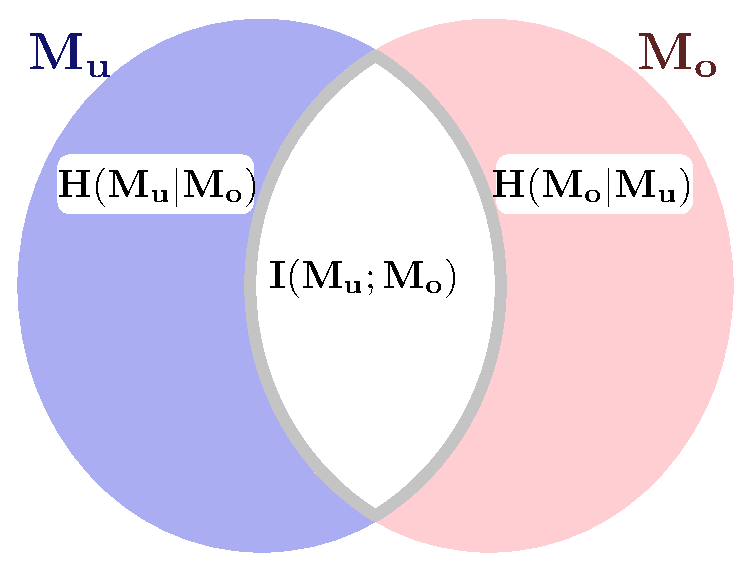
\includegraphics[width=0.35\textwidth]{chapters/cap-musicalidade/musicalidade-it.eps}
\caption{Informação mutua entre $M_u$ e $M_o$.}
\label{fig:InfoMutuaMuMo}
\end{figure}

Então seguindo a Definição \ref{def:MusicalidadeNaDancaIT} podemos afirmar que:
\begin{itemize}
\item $\mathbf{I(M_u;M_o):}$ é a informação mutua entre a música, $M_u$, e os movimentos, $M_o$.
$I(M_u;M_o)$ representa a quantidade de musicalidade na dança. 
\item $\mathbf{H(M_u|M_o):}$ é a informação que tem a música que não está nos movimentos.
Por exemplo, quando dançamos e a música está simplesmente de fundo, 
só sendo um elemento que emoldura os nossos movimentos sem afetar-lhos diretamente,
então teremos um caso de música incidental\footnote{A música incidental é muito utilizada no cinema, 
teatro, TV e video games; nestes âmbitos existe uma música de fundo que cria um ambiente para a cena \cite[pp. 17]{reinato2010musica} \cite[pp. 217]{dourado2004dicionario},
onde pouca informação da música está sendo usada, e esta serve só de marco emocional ou entrega uma informação além da ação na cena, para o espectador.}, e a informação musical não usada seria $H(M_u|M_o)$.
\item $\mathbf{H(M_o|M_u):}$ é a informação que tem os movimentos que não tem a música.
Por exemplo, se temos música incidental de caráter melancólica, e iniciamos a 
realizar movimentos em sequencia que representam a historia de nossa vida;
então a informação de nossa vida seria  $H(M_o|M_u)$.
\end{itemize}~

Finalmente, é interessante propor a seguinte pergunta e reflexão,
qual das danças mostradas na Figura \ref{fig:ex:infomutua} consideras com musicalidade?


\begin{figure}[ht]
\centering
\begin{subfigure}{.42\textwidth}
  \centering
  % include first image
  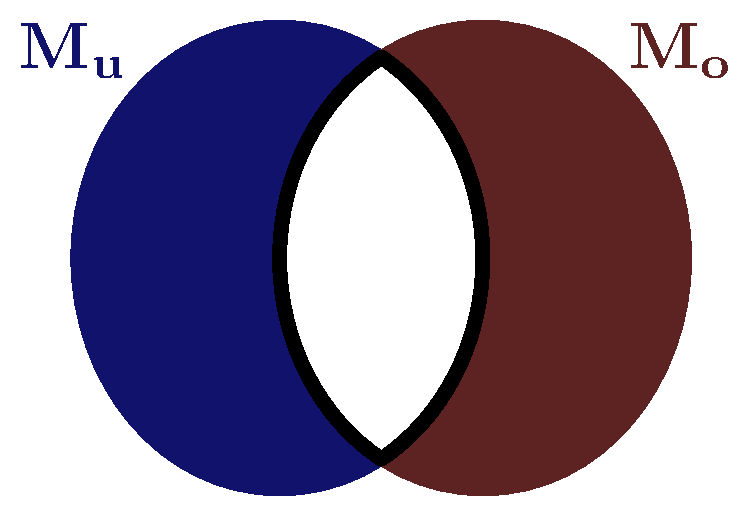
\includegraphics[width=.9\linewidth]{chapters/cap-musicalidade/musicalidade-it1.eps}  
  \caption{Caso 1.}
  \label{fig:ex:infomutua:a}
\end{subfigure}
\hfill	
\begin{subfigure}{.28\textwidth}
  \centering
  % include second image
  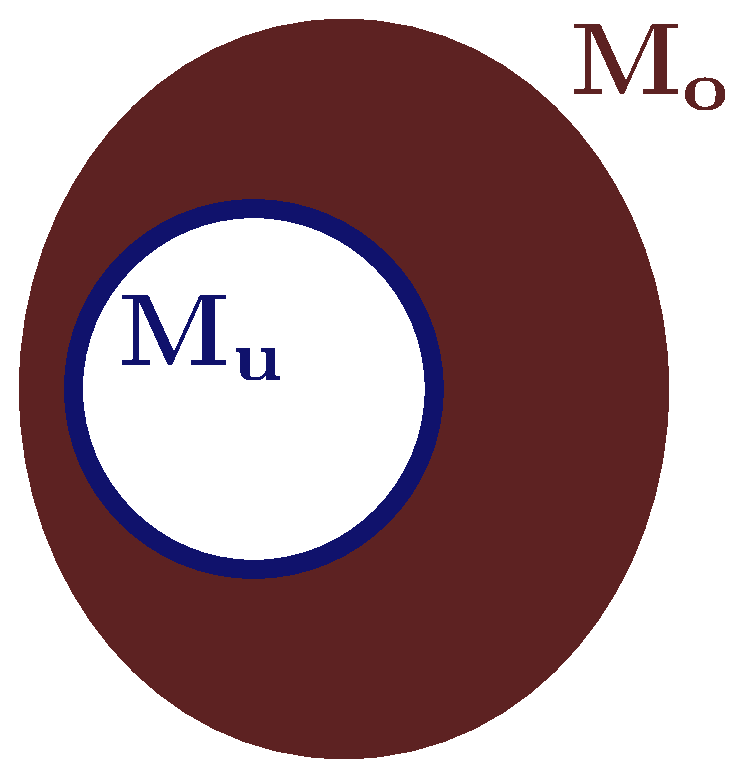
\includegraphics[width=.9\linewidth]{chapters/cap-musicalidade/musicalidade-it2.eps}  
  \caption{Caso 2.}
  \label{fig:ex:infomutua:b}
\end{subfigure}
\hfill
\begin{subfigure}{.28\textwidth}
  \centering
  % include second image
  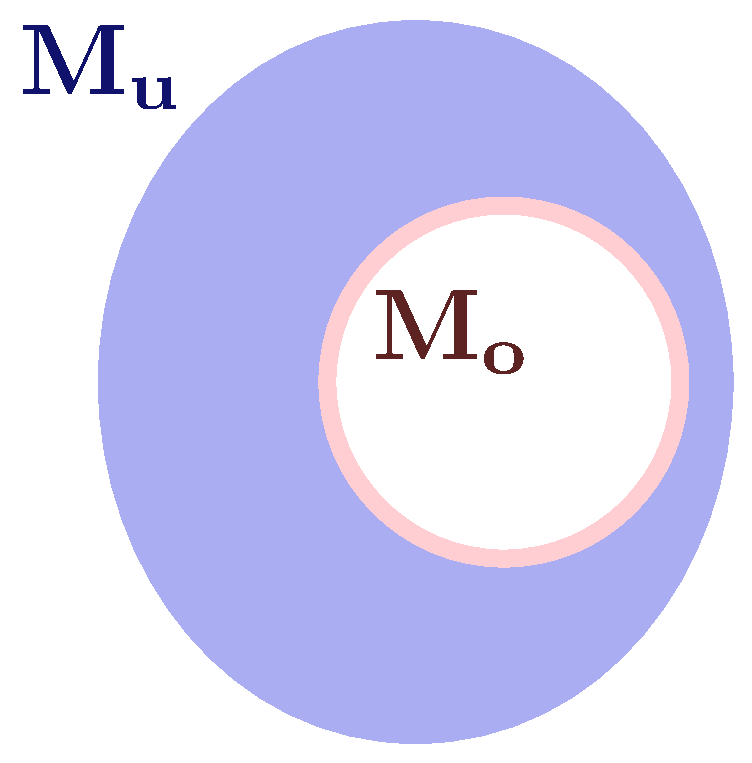
\includegraphics[width=.9\linewidth]{chapters/cap-musicalidade/musicalidade-it3.eps}  
  \caption{Caso 3.}
  \label{fig:ex:infomutua:c}
\end{subfigure}
\hfill
\begin{subfigure}{.52\textwidth}
  \centering
  % include first image
  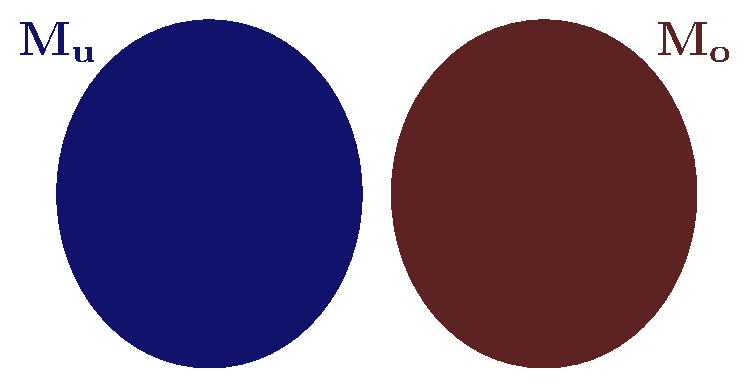
\includegraphics[width=.9\linewidth]{chapters/cap-musicalidade/musicalidade-type3.eps}  
  \caption{Caso 4.}
  \label{fig:ex:infomutua:d}
\end{subfigure}
\caption{Distintos tipos de usos da música na dança.}
\label{fig:ex:infomutua}
\end{figure}

Pessoalmente, eu me imagino:
\begin{itemize}
\item Na Figura \ref{fig:ex:infomutua:a} a um casal amigo meu dançando felizes.
\item Na Figura \ref{fig:ex:infomutua:b} escuto uma melodia simples, um solo de flauta,
fazendo em bucle uma frase de 4 compassos. 
Nessa música uma moça conta mediante a sua dança a historia da sua vida.
\item Na Figura \ref{fig:ex:infomutua:c} escuto uma música complexíssima, 
provavelmente polifônica, e um rapaz fazendo popping-dance,
onde cada um do seus movimento está atrelado às vontades de um instrumento na música.
\item Na Figura \ref{fig:ex:infomutua:d} me imagino a uma pessoa dançando de forma descompromissada com a música.
\end{itemize}


%%%%%%%%%%%%%%%%%%%%%%%%%%%%%%%%%%%%%%%%%%%%%%%%%%%%%%%%%%%%%%%%%%%%%%%%%%%%%%%%%
\begin{comment}
\subsection{\textcolor{red}{Relações da música com a dança}}
Em relação a como nossos movimentos são encaixados ou atrelados à música,
podem existir  3 tipos de relacionamento:
dependente, interdependente e independente \cite{butterworth2011dance}.

\begin{description}
\item[Dependente:] Este conceito de relação de dependência, entre música e dança, pode ter pelo menos 3 acepções.
    \begin{description}
    \item[Mickey mousing:]
    \item[visualização musical:]
    \item[Correlação direta:]
    \end{description}
\item[Interdependente:] Este é um termo usado para designar uma relação amigável,
entre música e dança; ou seja quando a música da um contexto onde se emoldura a dança,
porém esta tem liberdade de improvisar e contar historias dentro de uma estrutura definida, 
e usa a música como marco emocional e guia;
também pode-se referir ao caso quando, entre música e dança, 
se da uma relação de trabalho de pergunta e resposta, em ambos sentidos \cite{butterworth2011dance}. 
Este tipo de relação com a música está bem descrita pela Figura \ref{fig:ex:infomutua:a}.
\item[Indefinidamente:]
\end{description}
\end{comment}

%%%%%%%%%%%%%%%%%%%%%%%%%%%%%%%%%%%%%%%%%%%%%%%%%%%%%%%%%%%%%%%%%%%%%%%%%%%%%%%%
% https://translate.google.com.br/translate?sl=en&tl=pt&u=https%3A%2F%2Fthisdancinglife.com%2Fmusicality-in-dance%2F
